% -----------------------------------------------
% Template for ICMC SMC 2014
% adapted and corrected from the template for SMC 2013,  which was adapted from that of  SMC 2012, which was adapted from that of SMC 2011
% -----------------------------------------------

\documentclass{article}
\usepackage{icmcsmc2014}
\usepackage{times}
\usepackage{ifpdf}
\usepackage[english]{babel}
%\usepackage{flushend}
%\usepackage{cite}

%%%%%%%%%%%%%%%%%%%%%%%% Some useful packages %%%%%%%%%%%%%%%%%%%%%%%%%%%%%%%
%%%%%%%%%%%%%%%%%%%%%%%% See related documentation %%%%%%%%%%%%%%%%%%%%%%%%%%
%\usepackage{amsmath} % popular packages from Am. Math. Soc. Please use the
%\usepackage{amssymb} % related math environments (split, subequation, cases,
%\usepackage{amsfonts}% multline, etc.)
%\usepackage{bm}      % Bold Math package, defines the command \bf{}
%\usepackage{paralist}% extended list environments
%%subfig.sty is the modern replacement for subfigure.sty. However, subfig.sty
%%requires and automatically loads caption.sty which overrides class handling
%%of captions. To prevent this problem, preload caption.sty with caption=false
%\usepackage[caption=false]{caption}
%\usepackage[font=footnotesize]{subfig}


%user defined variables
\def\papertitle{Flocking: A Framework for Declarative Music-Making on the Web}
\def\firstauthor{Colin Clark}
\def\secondauthor{Adam Tindale}
\def\thirdauthor{nobody}
% adds the automatic
% Saves a lot of ouptut space in PDF... after conversion with the distiller
% Delete if you cannot get PS fonts working on your system.

% pdf-tex settings: detect automatically if run by latex or pdflatex
\newif\ifpdf
\ifx\pdfoutput\relax
\else
   \ifcase\pdfoutput
      \pdffalse
   \else
      \pdftrue
\fi

\ifpdf % compiling with pdflatex
  \usepackage[pdftex,
    pdftitle={\papertitle},
    pdfauthor={\firstauthor, \secondauthor},
    bookmarksnumbered, % use section numbers with bookmarks
    pdfstartview=XYZ % start with zoom=100% instead of full screen;
                     % especially useful if working with a big screen :-)
   ]{hyperref}
  %\pdfcompresslevel=9

  \usepackage[pdftex]{graphicx}
  % declare the path(s) where your graphic files are and their extensions so
  %you won't have to specify these with every instance of \includegraphics
  \graphicspath{{./figures/}}
  \DeclareGraphicsExtensions{.pdf,.jpeg,.png}

  \usepackage[figure,table]{hypcap}

\else % compiling with latex
  \usepackage[dvips,
    bookmarksnumbered, % use section numbers with bookmarks
    pdfstartview=XYZ % start with zoom=100% instead of full screen
  ]{hyperref}  % hyperrefs are active in the pdf file after conversion

  \usepackage[dvips]{epsfig,graphicx}
  % declare the path(s) where your graphic files are and their extensions so
  %you won't have to specify these with every instance of \includegraphics
  \graphicspath{{./figures/}}
  \DeclareGraphicsExtensions{.eps}

  \usepackage[figure,table]{hypcap}
\fi

%setup the hyperref package - make the links black without a surrounding frame
\hypersetup{
    colorlinks,%
    citecolor=black,%
    filecolor=black,%
    linkcolor=black,%
    urlcolor=black
}


% Title.
% ------
\title{\papertitle}

% Authors
% Please note that submissions are NOT anonymous, therefore
% authors' names have to be VISIBLE in your manuscript.
%
% Single address
% To use with only one author or several with the same address
% ---------------
%\oneauthor
%   {\firstauthor} {Affiliation1 \\ %
%     {\tt \href{mailto:author1@smcnetwork.org}{author1@smcnetwork.org}}}

%Two addresses
%--------------
 \twoauthors
   {\firstauthor} {OCAD University \\ %
     {\tt \href{mailto:cclark@ocadu.ca}{cclark@ocadu.ca}}}
   {\secondauthor} {OCAD University \\ %
     {\tt \href{mailto:atindale@faculty.ocadu.ca}{atindale@faculty.ocadu.ca}}}

% Three addresses
% --------------
% \threeauthors
%   {\firstauthor} {Affiliation1 \\ %
%     {\tt \href{mailto:author1@smcnetwork.org}{author1@smcnetwork.org}}}
%   {\secondauthor} {Affiliation2 \\ %
%     {\tt \href{mailto:author2@smcnetwork.org}{author2@smcnetwork.org}}}
%   {\thirdauthor} { Affiliation3 \\ %
%     {\tt \href{mailto:author3@smcnetwork.org}{author3@smcnetwork.org}}}


% ***************************************** the document starts here ***************
\begin{document}\sloppy
%
\capstartfalse
\maketitle
\capstarttrue
%
\begin{abstract}
Flocking\footnote{http://flockingjs.org/} is a framework for audio synthesis and music composition written in JavaScript. It takes a unique approach to solving several of the common architectural problems faced by computer music environments, emphasizing a declarative style that is closely aligned with the principles of the web.

In Flocking, instruments and scores are defined as JavaScript Object Notation (JSON) objects. JSON is a subset of the JavaScript language that is used widely across the web for exchanging data.\footnote{http://json.org} Flocking's goal is to enable the growth of an ecosystem of tools that can easily parse and understand the logic and semantics of digital instruments by representing the basic building blocks of synthesis declaratively. This is particularly useful for supporting generative composition (where programs generate new instruments and scores algorithmically), graphical tools (for programmers and non-programmers alike to collaborate), and new modes of social programming that allow musicians to easily adapt, extend, and rework existing instruments without having to ``fork" their code.

Flocking provides a robust, optimized, and well-tested architecture that explicitly supports extensibility and long-term growth. Flocking runs in nearly any modern JavaScript environment, including desktop and mobile browsers (Chrome, Firefox, and Safari), as well as on embedded devices with Node.js.

\end{abstract}

\section{Introduction}\label{sec:introduction}

A prominent stream in computer music research over the past few decades has focused on the creation of specialized languages for expressing musical and time-based constructs programmatically \cite{dannenberg2002language,wang2003chuck,mccartney1996supercollider,orlarey2009faust}. This emphasis on new forms of syntax and language-level expression has produced noteworthy computer music environments and useful results for many use cases such as live coding. Nonetheless, there is also a risk associated with the proliferation of isolated, specialist programming languages for music and art: an increased gap between creative coders and the resources available to mainstream software developers. For example, in many self-contained computer music environments, it continues to be difficult to create polished user interfaces or to connect with web-based services and sources of data---tasks that are routinely addressed in mainstream programming environments such as JavaScript. As artists and musicians increasingly use networked devices, sensors, and collaboration in their work, these limitations take an increasing toll on the complexity and scalability of creative coding.

Flocking is an open source JavaScript framework that aims to address some of these concerns by connecting musicians and artists with the cross-platform, distributed delivery model of the web, and with the larger pool of libraries, user interface components, and tutorials that are available to the web development community. Further, it emphasizes an extended approach to interoperability in which declarative instruments and compositions can be broadly shared, manipulated, and extended across traditional technical subcultural boundaries.

\subsection{Interoperability in Context}

A primary motivating concern for Flocking is that the tendency towards music-specific programming languages shifts focus away from interoperability amongst tools and systems. The term ``interoperability" is used here to describe a specific concept: the ability to share a single instance of a computer music artifact (i.e. an instrument or score) {\it bidirectionally} amongst human coders, generative or transformational algorithms, and authoring or graphical tools. Bidirectionality implies that a software artifact needs to preserve sufficient semantics and landmarks that it can be inspected, overridden, and extended by humans and programs not only at creation time but throughout the process of being used and maintained.

Today, a prospective computer musician often must choose from the outset whether or not she wants to use a code-based environment (such as SuperCollider or ChucK) or a graphical one (Max/MSP, Pd, or AudioMulch, for example). Since imperative programming code can't easily be parsed, generated, and understood by tools outside the chosen environment, the code and graphical paradigms rarely interoperate. This compounds the difficulty of collaborating on a musical project across modalities.

Interoperability amongst computer music systems has been addressed in a number of ways and to varying degrees. Open Sound Control \cite{wright1997open}, for example, helps support cross-system, message-based interoperability at runtime. Some graphical environments such as Max and Pd support the embedding of programmatic ``externals" within an otherwise graphical instrument. FAUST offers unidirectional code generators for a variety of target languages, enabling programs to be written in the FAUST language but deployed within other environments. The Music-N family's simple textual format has fostered a variety of third-party compositional tools that can process and generate score and orchestra files.

Some computer music environments also provide APIs for manipulating the language's parsing and compilation artifacts. One of CSound 6's new features includes an abstract syntax tree API, enabling a user to write C code that manipulates an orchestra prior to compilation \cite{fitch2013Csound6}. Max/MSP's Patcher API supports the programmatic traversal and generation of a Max patch using Java or JavaScript code\footnote{http://cycling74.com/docs/max5/vignettes/js/jspatcherobject.html}. Lisp-based languages such as Extempore go further towards potential interoperability, providing macro systems that allow for more robust generative algorithms to be created within the facilities of the language itself.

Within this context, Flocking aims to provide a framework that supports extended interoperability via a declarative programming model where the intentions of code are expressed as JSON data structures within the JavaScript language. This combines {\it metaprogramming} with an emphasis on publically-visible state and structural landmarks that help to support the alignment, sharing, and extension of musical artifacts across communities of programmers and tools.

\section{How Flocking Works}

\subsection{The Framework}

The core of the Flocking framework consists of several interconnected components that provide the essential behaviour of interpreting and instantiating unit generators, producing streams of samples, and scheduling changes. Flocking's primary components include:

\begin{enumerate}
\item the {\it Flocking interpreter}, which parses and instantiates synths, unit generators, and buffers
\item the {\it Environment}, which represents the overall audio system and its configuration settings
\item {\it Audio Strategies}, which are pluggable audio output adaptors (binding to backends such as the Web Audio API or ALSA on Node.js)
\item {\it Unit Generators} (ugens), which are the sample-generating primitives used to produce sound
\item {\it Synths}, which represent instruments and collections of signal-generating logic
\item the {\it Scheduler}, which manages time-based change events on a synth
\end{enumerate}

Figure \ref{fig:architecture} shows the runtime relationships between these components, showing an example of how multiple synths and unit generators are composed into a single Web Audio ScriptProcessorNode.

\begin{figure}[h]
\centering
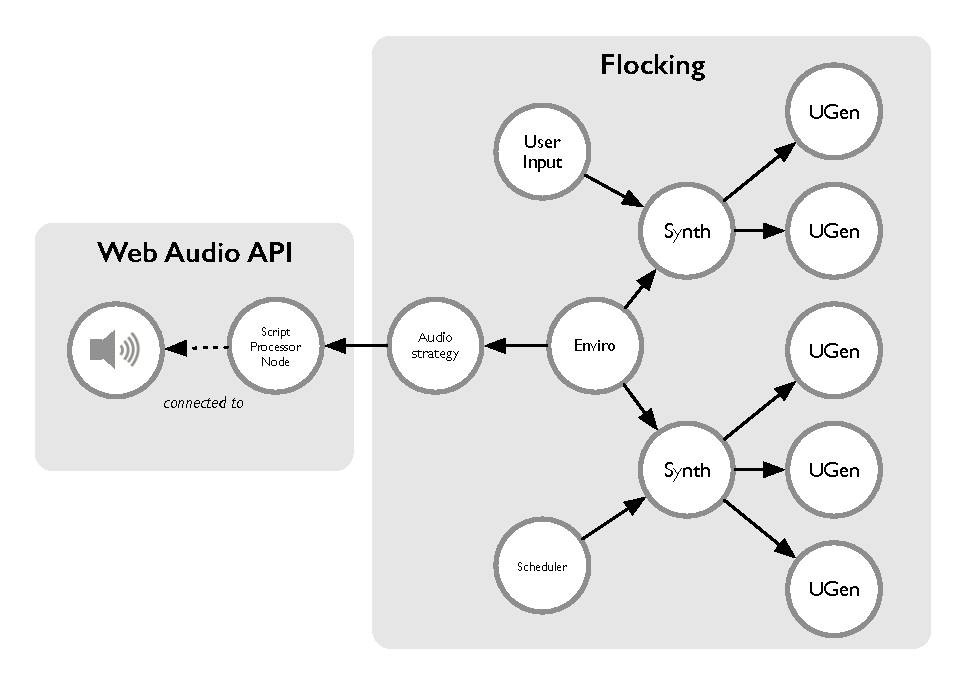
\includegraphics[width=0.9\columnwidth]{images/flocking-component-architecture.eps}
\caption{ A diagram showing Flocking's primary components and how they relate to each other and to the Web Audio API.\label{fig:architecture}}
\end{figure}

\subsection{Declarative Programming}

Above, we described Flocking as a declarative framework. This characteristic is essential to understanding its design. Declarative programming can be understood in the context of Flocking as having two essential aspects:

\begin{enumerate}
\item it emphasizes a high-level, semantic view of a program's logic and structure
\item it represents programs as data structures that can be understood by other programs
\end{enumerate}

J.W. Lloyd informally describes declarative programming as ``stating {\it what} is to be computed but not necessarily {\it how} it is to be computed" \cite{lloyd1994practical}. The emphasis here is on the logical or semantic aspects of computation, rather than on low-level sequencing and control flow. Traditional imperative programming styles are typically intended for an ``audience of one"---the compiler. Though code is often shared amongst multiple developers, it can't typically be understood or manipulated by programs other than the compiler.

In contrast, declarative programming involves the ability to write programs that are represented in a format that can be processed by other programs as ordinary data. The Lisp family of languages are a well-known example of this approach. Paul Graham describes the declarative nature of Lisp, saying it ``has no syntax. You write programs in the parse trees... [that] are fully accessible to your programs. You can write programs that manipulate them... programs that write programs." Though Flocking is written in ordinary JavaScript, it shares with Lisp the approach of expressing programs within data structures that are fully available for manipulation by other programs.

\subsection{JSON}

The key to Flocking's declarative approach is JSON, the JavaScript Object Notation format. JSON is a lightweight data interchange format based on a subset of JavaScript that can be parsed and manipulated in nearly any programming language. JSON provides several primary data types and structures that are available across programming languages. The following table describes these data structures and their syntax:

\begin{tabular}{| c || c | c |}
    \hline
    \bf{Type} & \bf{Syntax} & \bf{Description} \\ \hline
    Object & \verb|{}| & Dictionary of key/value pairs \\ \hline
    Array & \verb|[]| & An ordered list \\ \hline
    String & \verb|"cat"| & A character sequence \\ \hline
    Number & \verb|440.4| & A floating point number \\ \hline
\end{tabular}

Since JSON's syntax and semantics are identical to JavaScript's own type literals, JSON is a convenient language for representing data in web applications without imposing additional parsing complexity. All of Flocking's musical primitives are expressed as trees of JSON objects. These objects can be easily serialized, traversed, manipulated, and merged with other objects. In comparison to other music programming environments, which often describe themselves as functional or object-oriented, Flocking weaves the two approaches together in a manner that could be called ``document-oriented."

\subsection{Unit Generator Definitions}

Musicians working with Flocking don't typically instantiate unit generators directly. Instead, they compose JSON objects into trees. Each node in the tree, called a {\it unit generator definition} (ugenDef), describes a unit generator instance and its connection to others in the signal-processing graph. A ugenDef includes the following information:

\begin{enumerate}
\item the type of unit generator to be instantiated
\item a named set of inputs (key/value pairs), which can consist of either literal values (floats) or other unit generator specifications
\item the rate at which the unit generator will be evaluated (audio, control, or constant); this defaults to \verb|"audio"| if omitted
\item a named set of static options, which describe how the unit generator should be configured
\end{enumerate}

Below is a simple example of a sine wave oscillator, illustrating how Flocking unit generators are defined in JSON:

\begin{verbatim}
{
  ugen: "flock.ugen.sinOsc",
  rate: "audio",
  inputs: {
    freq: 440,
    mul: 0.25
  },
  options: {
    interpolation: "linear"
  }
}
\end{verbatim}

Unit generator types are expressed as dot-separated strings called {\it key paths} or {\it EL expressions}. These strings are bound to creator functions at instantiation time by Flocking. All type expressions refer to a global namespace hierarchy so that developers can easily contribute their own unit generator implementations (using their own namespace to avoid conflicts) and have the Flocking framework manage them in the same manner as any of the built-in types.

\subsection{Synth Definitions}

A collection of unit generator definitions form the basis of a {\it synth definition} (synthDef). Synth definitions describe a complete instrument to be instantiated by the Flocking framework. Synths typically include a connection to an output bus---either the speakers or one of the environment's shared ``interconnect" buses. In this respect, Flocking's architecture is inspired by the SuperCollider server \cite[pp.25]{wilson2011supercollider}. Here is a simple example of a synthDef that outputs two sine waves, one in each stereo channel:

\begin{verbatim}
{
  ugen: "flock.ugen.out",
  sources: [
    {
      ugen: "flock.ugen.sinOsc"
    },
    {
      ugen: "flock.ugen.sinOsc",
      freq: 444
    }
  ]
}
\end{verbatim}

This example also illustrates a key aspect of Flocking's interpreter and its document-merging approach. In the case of the first unit generator, we have omitted all input values. When the synth is instantiated, it will automatically be given a frequency of 440 Hz and an amplitude of 1.0. This is due to the fact that every built-in unit generator declares a set of default values. The Flocking interpreter, prior to instantiating the unit generator, will merge the user's ugenDef values on top of the defaults. If a property is omitted, the default value will be retained; if a user specifies a property, it will be used in place of the default. To save typing, the interpreter will also handle input names correctly when they aren't nested inside an ``inputs" container. Notably, this defaulting and permissiveness is implemented in a publicly visible way (as JSON {\it defaults specifications}), helping to ensure that these programming conveniences wont't restrict interoperability with other tools.

To instantiate a Synth, its creator function must be called. In Flocking, a component creator function typically takes only one argument---the component's {\it options} structure---and returns an instance of the component. For all synths, the options object must include a synthDef as well as any other settings needed to appropriately configure the synth instance. Figure \ref{fig:pmSynth} shows how a Flocking synth is created programmatically.

\begin{figure}[h!]
    \begin{verbatim}
var synth = flock.synth({
  synthDef: {
    id: "carrier",
    ugen: "flock.ugen.sinOsc",
    freq: 440,
    phase: {
      id: "mod",
      ugen: "flock.ugen.sinOsc",
      freq: 34.0,
      mul: {
        ugen: "flock.ugen.sinOsc",
        freq: 1/20,
        mul: Math.PI
      },
      add: Math.PI
    },
    mul: 0.25
  }
});
    \end{verbatim}
    \caption{Instantiating a custom phase modulation synth.\label{fig:pmSynth}}
\end{figure}

By default, synths are automatically added to the tail of the Environment's list of nodes to evaluate, so they will start sounding immediately if the Environment has been started.

\subsection{Updating Values}

Once a synth has been instantiated, its inputs can be changed on the fly. Flocking supports a highly dynamic signal processing pipeline; unit generators can be added or swapped out from a synth at any time, even while it's playing. Behind the scenes, everything in the signal graph is a unit generator, even static values.

In order to direct changes at a particular unit generator, it has to be given an identifying name. In the example shown in figure \ref{fig:pmSynth}, the carrier and modulator unit generators are each given an \verb|id| property that exposes them publicly. These names represent ``cutpoints" into the overall tree that provide easier access to a particular unit generator. Synths keep track of all their named unit generators and provide \verb|get| and \verb|set| methods for making programmatic changes to their inputs.

Changes can be targeted at any unit generator within the tree using key path expressions. Here is an example of how changes can be made to different points in the unit generator tree with a single call to \verb|Synth.set()|:

\begin{verbatim}
  synth.set({
    "carrier.freq": 220,
    "mod.mul.freq": 1/30
  });
\end{verbatim}

This example lowers the frequency of the carrier oscillator by an octave while simultaneously slowing down the rate at which the modulator's amplitude is oscillating.

This hierarchical path-based scheme for addressing Flocking's graph of signal generators is inspired by Open Sound Control's {\it addresses}, which provide a similar means for specifying arbitrary message targets within a tree. Indeed, OSC messages can be easily adapted to Flocking change specifications; this is accomplished with only a few lines of code in the Flocking OSC library.\footnote{https://github.com/colinbdclark/flocking-osc/}

\section{Scheduling} \label{sec:Scheduling}

\subsection{Unit Generators Represent Change}

Modelling the architectural distinction between different types of changes that occur at varying time scales is a common challenge faced by computer music systems. Such changes include:

\begin{enumerate}
\item highly optimized data flow-based changes that occur at the signal level
\item value or instrument changes scheduled at fixed or indeterminate rates (a ``score")
\item messages or events sent between objects in an object-oriented system
\item user-triggered events from an OSC or MIDI controller, or from graphical user interface components such as buttons and knobs
\end{enumerate}

Different systems take markedly different approaches to modelling these distinctions. Flocking attempts to unify the means for expressing both micro- and macro-level changes in a composition. Where other systems create a fundamental semantic and syntactic distinction between different sources of change (e.g. unit generators vs. patterns in SuperCollider), instruments and scheduled events alike are specified in Flocking as a tree of unit generators. The primary difference is the rate at which these unit generators are evaluated. This allows the same instruments that are used to define the note-level timbre and texture of a piece to be reused when shaping the larger-scale phrasing and structure of the music.  Figure \ref{fig:schedulerEx} provides an example of how changes are scheduled using Flocking's declarative scheduler to create a simple drum machine.

\begin{figure}[h!]
    \begin{verbatim}
flock.scheduler.async.tempo({
  bpm: 180,

  score: {
    interval: "repeat",
    time: 1,
    change: {
      synth: "drumSynth",
      values: {
        "trig.source": {
          synthDef: {
            ugen: "flock.ugen.sequence",
            list: [
              1, 1, 0, 1,
              1, 0, 1, 0
            ],
            loop: 1
          }
        }
      }
    }
  }
});
    \end{verbatim}
    \caption{Scheduling changes with the Flocking Scheduler.\label{fig:schedulerEx}}
\end{figure}

This example assumes that there is already a synth running (named ``drumSynth"), which will produce a drum sound whenever its trigger input changes. First, we instantiate an asynchronous tempo scheduler---a type of scheduler that runs outside of the sample generation pipeline and that accepts time values specified in beats per minute. Currently there are only asynchronous Schedulers in Flocking; a sample-accurate implementation is in the planning stages.

The details of the desired changes are specified in the ``score" section of the example. This particular score is defined with the following parameters:

\begin{itemize}
\item it should be repeatedly applied, every beat
\item each change should be targeted at a particular instrument (specified by name)
\item the value of each change should be determined by evaluating the supplied synthDef
\end{itemize}

In Flocking, synths can be evaluated at different rates, including at audio, control, scheduled, and demand rate. The scheduler automatically takes care of parsing the JSON-based {\it change specification}, producing a {\it value synth} running at the specified scheduled rate, and targeting its stream of changes to the desired instrument synth. In figure \ref{fig:schedulerEx} above, the scheduled synth will be evaluated on every beat. It produces values using a simple \verb|sequence| unit generator, which cycles through a list of numbers in order.

\begin{figure}[ht]
\centering
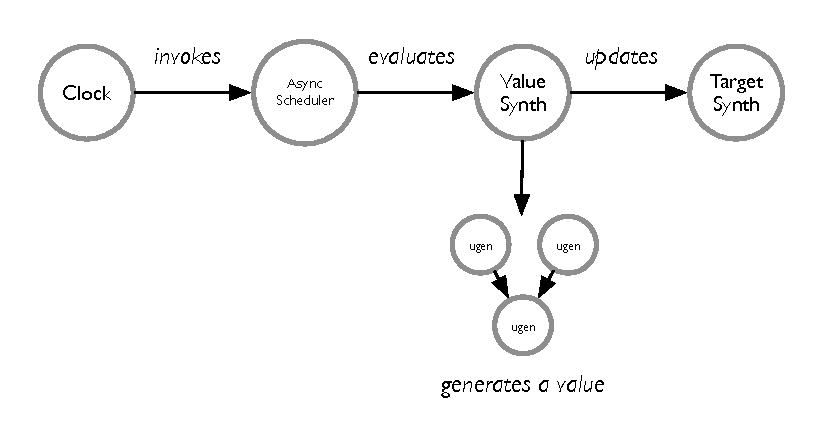
\includegraphics[width=0.9\columnwidth]{images/scheduler.eps}
\caption{ Diagram showing the runtime structure of Flocking's declarative scheduler.\label{fig:scheduler}}
\end{figure}

A full version of the example in figure \ref{fig:schedulerEx}, which also illustrates how synths and schedulers can be woven together in an entirely declarative way, is available on Github\footnote{https://github.com/colinbdclark/flocking-examples/blob/master/drum-machine/drum-machine.js}.

\subsection{Rationale}

This approach was inspired by an insight in James Tenney's {\it Computer Music Experiences} \cite{tenney1969computer}, where he points out the conceptual similarity between the macrostructure of a composition---events that occur over the duration of a piece of music---and the changes that occur at the microlevel of unit generators. In the early 1960s, Tenney attempted to use Music IV's unit generator system as the basis for algorithmically specifying the large-scale time structure of his compositions. He commented that the instruments ''produced results that were quite interesting to me, but it was not very efficient to use the compiler itself for these operations\ldots [requiring] a separation between the compositional procedures and the actual sample-generation" \cite[p.41--42]{tenney1969computer}. This suggests that the architectural rift between composition-level and signal-level changes, which has been inherited by several generations of computer music systems since the 1960s, was born out of early performance issues.

Few would doubt that the performance factors of today's computer music systems are the same as they were on early mainframe systems, and the elegance and power of using unit generator for both signal- and composition-level changes is worth revisiting. Aside from simplicity, one of the main advantages of Flocking's approach to declarative scheduling is that it offers the potential to actually improve performance in the long run. A typical problem with computer music schedulers is ensuring that whatever work a user schedules is deterministic and optimized for real-time performance. Schedulers either have to trade off expressivity, limiting the types of changes that can be scheduled (such as with the Web Audio API's AudioParams), or leave it entirely up to the user to implement event producers that are sufficiently optimized. Flocking attempts to help users express changes in a way that can be optimized automatically by the framework. Unit generators are explicitly designed to be used in a real-time constrained context. As a result, the Flocking interpreter is free to take a scheduled synthDef and, if appropriate, inject its unit generator tree directly into the signal path of the target synth, ensuring that all changes occur with as little overhead as possible.

SynthDefs are similarly used in Flocking's MIDI and OSC libraries to define transformations between incoming control values and the inputs of an audio synth.

\section{Current State}

\subsection{Relationship to the Web Audio API}

Flocking currently makes limited use of the built-in native audio processing nodes in the W3C's Web Audio API\footnote{http://www.w3.org/TR/webaudio/}. It is the opinion of the authors that the version of the Web Audio API shipping in browsers today is insufficient to support the expressivity required by creative musicians without the support of additional libraries. Many of the limitations of the API are outlined in detail in \cite{DBLP:journals/comj/WyseS13}. Web Audio currently provides limited options for web developers who want to create their own custom synthesis algorithms in JavaScript and expect them to perform well. In particular, it is difficult to mix native and JavaScript-based nodes in the same signal graph without imposing latency and synchronization issues.

Flocking predates the first Web Audio API implementation, and was architected specifically to allow web developers to contribute their own first-class signal processing implementations in an open way. As a result of this philosophy, and due to the performance and developer experience issues of the current Web Audio specification, Flocking uses only small parts of the API. Instead, it takes full control of the sample-generation process and provides musicians with an open palette of signal-generating building blocks that can be used to assemble sophisticated digital instruments.

\subsection{Comparison with Web Audio Libraries}

Several other libraries also take a similar ``all JavaScript" approach. {\it Gibberish} \cite{roberts_web_2013} and {\it CoffeeCollider} \cite{Mohayonao} are two prominent alternatives to Flocking. CoffeeCollider attempts to replicate the SuperCollider environment as closely as possible using the CoffeeScript programming language \cite{Ashkenas}, while Gibberish takes a more traditional object-oriented approach. Although these environments each offer their own unique features, neither has attempted to stray far from the conventional models established by existing music programming environments.

Flocking, too, has taken architectural inspiration from several existing music programming systems, particularly the design of the SuperCollider 3 synthesis server. Flocking shares with it a simple ``functions and state" architecture for unit generators, as well as a strict (conceptual) separation between the realtime constraints of the signal-processing world and the more dynamic and event-driven application space, manifested in the architectural distinction between unit generators and synths \cite[pp. 64]{mccartney2002rethinking}.

\subsection{Performance}

Much has been written about web audio performance issues related to the current generation of JavaScript runtimes generally (lack of deterministic, incremental garbage collection) and the Web Audio API specifically (the requirement for ScriptProcessorNodes to run on the main browser thread) \cite{DBLP:journals/comj/WyseS13,roberts_web_2013}. If history is any indication, it seems likely that the performance characteristics of the JavaScript language will keep improving as the browser performance wars continue to rage between Mozilla, Google, and Apple. In addition, Web Worker-based strategies for sample generation are currently being discussed for inclusion in the Web Audio API specification\footnote{https://github.com/WebAudio/web-audio-api/issues/113}, which will significantly improve the stability of JavaScript-based signal generators.

In the interim, many claims have been made about the relative performance merits of various optimization strategies used in toolkits such as Gibberish \cite{roberts_web_2013}. Most of these claims, however, focus on micro-benchmarks that measure the cost of small-scale operations in isolation, rather than taking into account the performance of real-world signal processing algorithms.

Avoiding the temptation to focus on micro-benchmarking and premature optimization, the approach we have taken in Flocking is to build an architecture and framework that can serve as a flexible, long-term foundation on which to continually evolve new features and improved performance. Significant effort has been invested in developing automated unit and performance tests for Flocking that measure the real-world costs of its approach.

\begin{figure}[ht]
\centering
\includegraphics[width=0.9\columnwidth]{images/FlockingVsGibberish20ptFont.pdf}
\caption{ A comparison of performance between Flocking and Gibberish. Smaller bars are faster. \label{fig:flockingvsgibberish}}
\end{figure}

With just-in-time compilers such as Google's V8\footnote{https://code.google.com/p/v8/} and Mozilla's IonMonkey\footnote{https://wiki.mozilla.org/IonMonkey/Overview}, we believe that real-world performance is best achieved by using simple algorithms that represent stable ``hot loops" that can be quickly and permanently  compiled into machine code by the runtime. The risk of micro-optimization efforts such as the code-generation techniques promoted by Gibberish is ``lumpy" (i.e. of an unpredictable duration) real-world performance caused by the JavaScript runtime having to re-trace and recompile code. This is particularly an issue when code needs to be dynamically generated and evaluated whenever the signal graph changes, such as the introduction of new synths or unit generators into the pipeline. Flocking avoids this risk while maintaining competitive performance by using a simple algorithm for traversing and evaluating unit generators. Synth nodes and unit generators are stored in flat, ordered lists. Flocking is able to quickly iterate through these lists and evaluate each signal generator in order. Synth nodes and unit generators can be added or removed from the pipeline at any time without forcing the JavaScript runtime to spill its caches when evaluating a new piece of code. This helps to ensure that Flocking's performance profile remains stable and consistent at runtime.

Despite very little optimization effort to date, preliminary benchmarks\footnote{https://github.com/colinbdclark/webaudio-performance-benchmarks} suggest that Flocking's approach is promising both from the perspective of good performance as well as greater simplicity and maintainability in comparison to systems that use more complex code generation techniques. Figure \ref{fig:flockingvsgibberish} shows a simple test where one second's worth of samples were generated and timed for an FM synth consisting of three sine oscillators. This test was performed 10000 times to illustrate realistic VM behaviour. The minimum, average, and maximum times are graphed in milliseconds. The tests were carried out on an Apple MacBook Pro laptop with a 2.3 GHz Intel Core i7 processor. Many factors can influence benchmark results, but Flocking's performance appears to be significantly better than Gibberish on every browser.

\subsection{The Flocking Playground}

Flocking's data-oriented approach can be useful for a variety of musical and social purposes. For example, a generative music application can algorithmically produce JSON synthDefs on the fly that introduce new instruments or variations on existing instruments into the system. Similarly, a visualization and editing environment can traverse the source code of a synthDef and produce a rendering that allows users to inspect or edit their instruments visually.

The Flocking Playground (see figure \ref{fig:playground}) is a simple web-based development environment that serves as an evolving platform for showing Flocking's features and approach. It provides the ability to:

\begin{itemize}
\item browse, audition, edit, and share links to a variety of Flocking demos
\item develop new instruments and compositions in the integrated code editor
\item see a synchronized visual rendering of a synth's source code
\end{itemize}

The Playground's graphical mode parses a user's JSON SynthDef specifications and renders them on the fly using a combination of HTML, CSS, and SVG into a flow-based diagram that illustrates the synth's structure and signal flow.

\begin{figure}[ht!]
\centering
\includegraphics[width=0.9\columnwidth]{images/flocking-playground-source-view.png}
\caption{ A screenshot of Flocking's interactive programming environment.\label{fig:playground}}
\end{figure}

\begin{figure}[ht]
\centering
\includegraphics[width=0.9\columnwidth]{images/flocking-playground-graphical-view.png}
\caption{ A screenshot of the Playground's visual view.\label{fig:graphical}}
\end{figure}

The Flocking Playground is built with Fluid Infusion\footnote{http://fluidproject.org/products/infusion}, a JavaScript framework that supports end-user personalization and authoring \cite{hcii2014}. Infusion's infrastructure for relaying, transforming, and firing changes across diverse models within an application are critical for maintaining synchronization between the graphical and source views of the Playground. Infusion continues to be a source of significant architectural inspiration for Flocking, and the two frameworks share a common philosophy and approach.

\subsection{Greater Web Audio Integration}

Due to the fact that Flocking takes control of the sample generation process directly, it uses very few features of the W3C Web Audio API. As the specification evolves, plans are underway to adopt more of its features in Flocking. At the moment, Flocking consists of a single ScriptProcessorNode that is connected to the Web Audio API's destination sink. Limited support for injecting native Nodes before and after the Flocking script node is available, opening up the possiblity of using nodes such the MediaStreamSource, Panner, and Analyser nodes in tandem with Flocking. Nonetheless it remains difficult to build complex graphs that mix native and Flocking-based processors.

We are in the midst of planning an updated version of the Flocking architecture that allows Flocking unit generators to be interleaved freely with native Web Audio nodes. This approach will introduce a proxy unit generator type that adapts inputs between a native node and a Flocking unit generator.

\begin{figure}[ht]
\centering
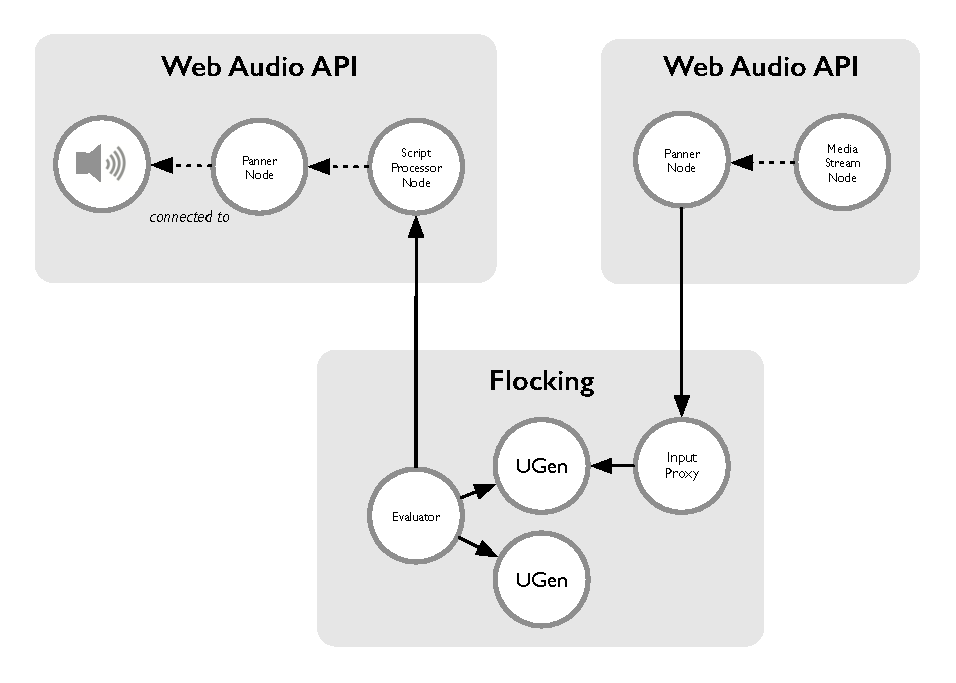
\includegraphics[width=0.9\columnwidth]{images/flocking-web-audio-islands.eps}
\caption{ A diagram showing how Flocking will support mixing unit generators with native Web Audio API nodes.\label{fig:webaudioflocking}}
\end{figure}

This architecture change will also help prepare Flocking for Web Worker-based ScriptProcessorNodes, which are planned for a future version of the Web Audio specification\footnote{https://github.com/WebAudio/web-audio-api/issues/113}.

\section{Conclusions}

Flocking is a new framework for computer music composition that leverages existing technologies and ideas to create a robust, flexible, and expressive system. Flocking combines the unit generator pattern from many canonical computer music languages with Web Audio technologies to allow users to interact with existing and prospective web technologies. Users interact with Flocking using a declarative style of programming.

The benefit of Flocking's approach, when considering various examples of web development environments using both text and visual idioms, has been demonstrated. Flocking provides users with a clear and semantic way to represent the materials of digital music, a promising framework for growing new features and tools, and a light performance footprint.


%%%%%%%%%%%%%%%%%%%%%%%%%%%%%%%%%%%%%%%%%%%%%%%%%%%%%%%%%%%%%%%%%%%%%%%%%%%%%
%bibliography here
\bibliography{flockingbibliography}

\end{document}
